%\documentclass{cwparticle} % for review/editing/polishing
%\linespread{1.5}           % for review/editing/polishing
\documentclass[onecolumn]{cwpreport} % for final draft


% Packages used by default CWP reports built by M8R
\usepackage{times,natbib,amsmath,graphicx,color,amssymb,amsbsy,lineno,setspace,algorithm2e,lipsum}

% Specific paper formatting for CWP report
\setlength{\paperwidth}{8.5in}
\setlength{\paperheight}{11.0in}
\setlength{\topmargin}{-0.25in}
\setlength{\textheight}{8.75in}
\setlength{\textwidth}{6.5in}
\setlength{\oddsidemargin}{+.015625in}
\setlength{\evensidemargin}{+.015625in}

% Final draft only
\title[Short Title]{I Wish I Could Come Up With A More Creative Title} 
% for editing/reviewing
%\title{Measuring wave propagation through an open-pit mine using stereo videos} 
%\righthead{training data}
%\lefthead{Rapstine & Sava}

% Final draft only
\author[Author1  \& Author2]{Jane Author1 \& John Author2 
\\
Center for Wave Phenomena and Dept. of Geophysics, Colorado School of Mines, Golden CO 80401 \\ email author1@mines.edu} 
%
%\author{Thomas Rapstine, Paul Sava, Ashley Grant, \& Jeff Shragge}
\begin{document}

\maketitle

% Uncomment for final draft only
%\setcounter{page}{285}
\journal{CWP-999}

%% ------------------------------------------------------------
\begin{abstract}
\lipsum[2]
\end{abstract}
%% ------------------------------------------------------------

% Uncomment for final draft only
%% ------------------------------------------------------------
\begin{keywords}
Keyword1, Keyword2, Keyword3 
\end{keywords}
%% ------------------------------------------------------------

%% ------------------------------------------------------------
\section{Introduction}
\lipsum[2-4]

Here is an example of an citation \citep{hale_atomic_2001}. Here is an example of an inline citation from \cite{haber_inversion_2007}.

%% ------------------------------------------------------------

%% ------------------------------------------------------------
\section{Theory}
\lipsum[2-4]

And now for some theory:

\begin{equation}
	(x+3)(x+2)=x^2+5x+6 \geq x^2
\end{equation}


\begin{figure}
    \centering
    
\includegraphics[width=0.6\textwidth]{Fig/CWP-logo-alpha.jpg} 
    \caption{Here is the CWP logo.}
    \label{fig:model_map}
\end{figure}

%% ------------------------------------------------------------

%% ------------------------------------------------------------
\section{Experiments}
\lipsum[2-4]
\begin{figure}
    \centering
    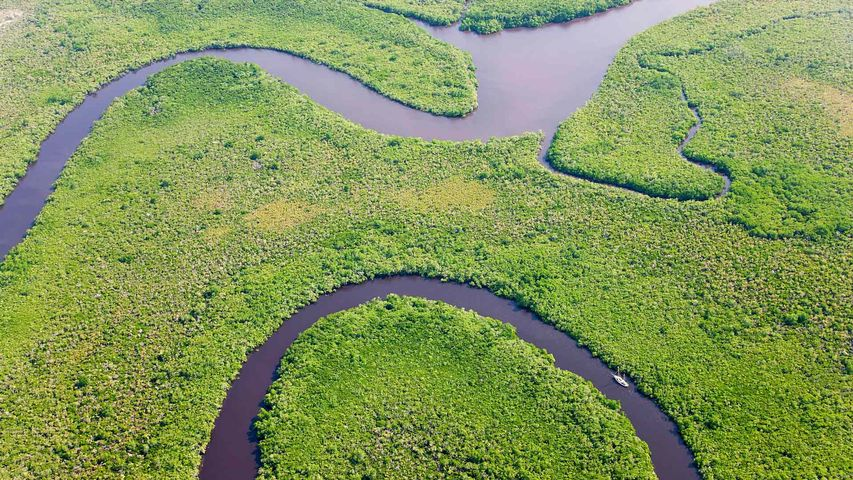
\includegraphics[width=0.475\textwidth]{Fig/DaintreeRiver.jpg}  
    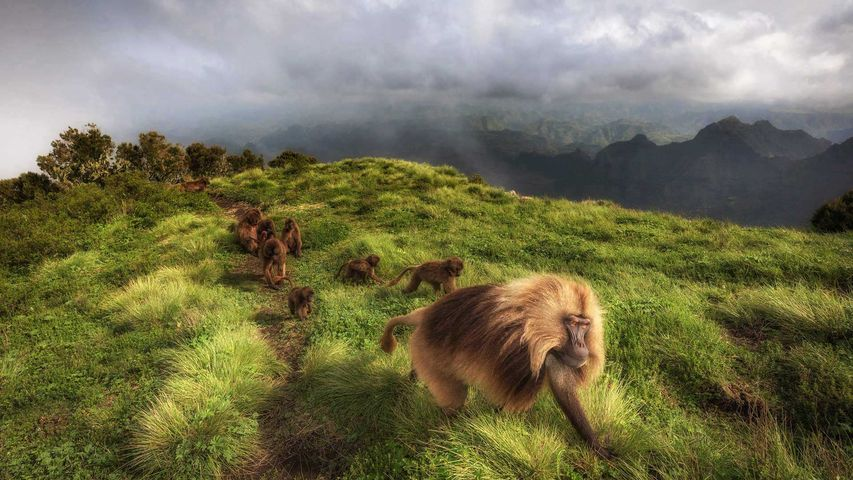
\includegraphics[width=0.475\textwidth]{Fig/GeledaMonkeys.jpg} 
    \caption{Photo of the (a) Daintree River in Australia and (b) the Geleda Monkeys.}
    \label{fig:model_volume}
\end{figure}
%% ------------------------------------------------------------

%% ------------------------------------------------------------
\section{Discussion}
\lipsum[2-4]
%% ------------------------------------------------------------

%% ------------------------------------------------------------
\section{Conclusions}
\lipsum[2-4]
%% ------------------------------------------------------------

%% ------------------------------------------------------------
\section{Acknowledgements}
We thank the sponsor companies of the Center for Wave Phenomena,
whose support made this research possible.
%% ------------------------------------------------------------

%% ------------------------------------------------------------
%\newpage
\bibliographystyle{seg}
\bibliography{references}
%% ------------------------------------------------------------

%% ------------------------------------------------------------


%% -----------------
\end{document}